\chapter{Японски имена}
\label{chap:imena}
\section{Основни правила при транскрипцията на японски имена}
\subsection{Дългите гласни}
В практическата транскрипция е прието \textbf{дължината на гласните} да не се предава.
Когато обаче йероглифният запис на \textbf{съответното име} или \textbf{термин} е даден в скобки, той може да бъде \textbf{транскрибиран на кирилица}, като се отрази и дължината на гласните.
Затова например глинените фигурки от \textit{периода Джьомон} в текста се срещат като \textit{догу}, но йероглифният запис е транскрибиран като \textit{догуу}.

Аналогичен е случаят и с термина \textit{шинто}, който всъщност звучи като \textit{шинтоо}.
При необходимост предаването на дългите гласни може да стане по няколко начина: чрез повторно изписване на съответната гласна; чрез чертица над буквата; чрез двоеточие след нея. Така дългата гласна \textbf{/a/} може да се срещне като \textbf{/aa, \-а, a:/}.
В англоезичната литература е разпространено и предаването на дължината с помощта на буквата h. Така например названието на \textit{японския театър Но}, което в действителност звучи \textbf{/ноо/},
на английски се транскрибира като \textbf{Noh}.

\subsection{Редукция на гласните}
Типична за японския език е редукцията на тесните гласни \textbf{/u, i/} в неударени срички и в края на думите, както е например в \textbf{копулата /десу/} и в \textbf{суфикса /масу/}.
Тъй като в тези случаи \textbf{редукцията} е почти пълна, при предаване на японски имена с наставка \textbf{суке}, е по-добре тя да се изписва като \textbf{ске}, т.е \textit{Дайске}, а не \textit{Дайсуке}.

\subsection{Двойните съгласни}
Двойните съгласни се предават при свързването на \textbf{две морфеми} и при т.нар. \textbf{експресивна геминация}. Името на страната може да бъде произнесено или като \textit{Нихон}, или като \textit{Ниппон}, но не и като \textit{Нипон}. Важно е да се знае, че \textit{Нихон} и \textit{Ниппон} не са напълно взаимозаменяеми.
Например в спортни призиви при международни мачове се използва \textit{„Ниппон – Ганбаре Ниппон“}!

В японския се среща\textbf{ удвояване на съгласните}, което в английската транскрипция се отбелязва
просто с \textbf{удвоение на буквите}, като например \textbf{"kk"}, \textbf{"tt"}. Това се прави и в българската транскрипция. Т.е. в такива случаи се транслитерира буквално - \textbf{tt = тт, kk = кк}, и т.н.

\subsection{Морообразуващата съгласна /н/}
В японски език се срещат \textbf{два вида съгласни /н/}. Едната не се различава от българската и в позиция пред букви, предаващи йотувани гласни, се смекчава. Другата, която се записва с буквата \begin{CJK*}{UTF8}{song}ん\end{CJK*}, е т.нар. \textbf{морообразуваща съгласна /н/}, която винаги се \textbf{произнася като} \textbf{твърда}. В английската транскрипция този звук се предава чрез \textbf{апостроф (n’),} както в заглавието на антологията \textbf{Man’y\-osh\-u}, ако е отразена дължината на гласните, и като \textbf{Man’yoshu}, ако не е отразена.
В руската транскрипция се използва буквата \textbf{\"e}, която се нарича \textbf{твердый знак} и при необходимост изпълнява ролята на \textbf{апостроф}, както например в \textbf{Манъ\"eсю}.
В българската азбука \textbf{ъ} има самостоятелна звукова стойност и не може да се използва като апостроф. Тъй като употребата на апостроф, макар и с по-други функции, се допуска от българския правопис, тук ще го използвам в съчетание с буквата \textbf{н} за предаване на морообразуващата съгласна, както например \textbf{Ман’йошю}.

\subsection{Меките ж, ч, ш}
Българският правоговор изисква съгласните \textbf{ж, ч, ш} да се произнасят като \textbf{твърди}, но в японския език те са \textbf{меки съгласни}. Сричката 
\begin{CJK*}{UTF8}{song}しゅ\end{CJK*} например се предава или като \textbf{шу} под влияние на английската транскрипция, или като \textbf{сю} под влияние на руската. По-близо до японското произношение обаче е \textbf{шю}. Ето защо името на най-големия японски остров например е \textbf{Хоншю}, а не \textbf{Хоншу} или \textbf{Хонсю}.

\subsection{Дзен или зен}
Под влияние на \textbf{английската транскрипция} често се пише \textbf{з} вместо \textbf{дз}, като дори се твърди, че това е правилното произношение. Ако обаче привържениците на това твърдение помолят някой японец да произнесе например думата \textbf{защо}, със сигурност ще чуят \textbf{дзащо}.

\subsection{Сричката /цу/}
Африкатата \textbf{/ц/,} която се среща в японската сричка \textbf{/цу/,} при транскрипция с латиница се предава с буквосъчетанието \textbf{/ts/.} Тъй като този звук не се различава от българския \textbf{/ц/,} \textbf{при} \textbf{транскрибирането} му не би трябвало да има колебания.
Но авторите, които \textbf{механично следват английската транскрипция}, често пишат или\textbf{ тс, }или\textbf{ }дори\textbf{ тц}. Така \textbf{Цукуба} се среща и като \textbf{Тсукуба}, и като \textbf{Тцукуба}. \\\\

\textbf{Източник:} „\textbf{\textit{Японската цивилизация}}“ от Братислав Иванов.
 
\begin{table}[htbp]
    \centering
    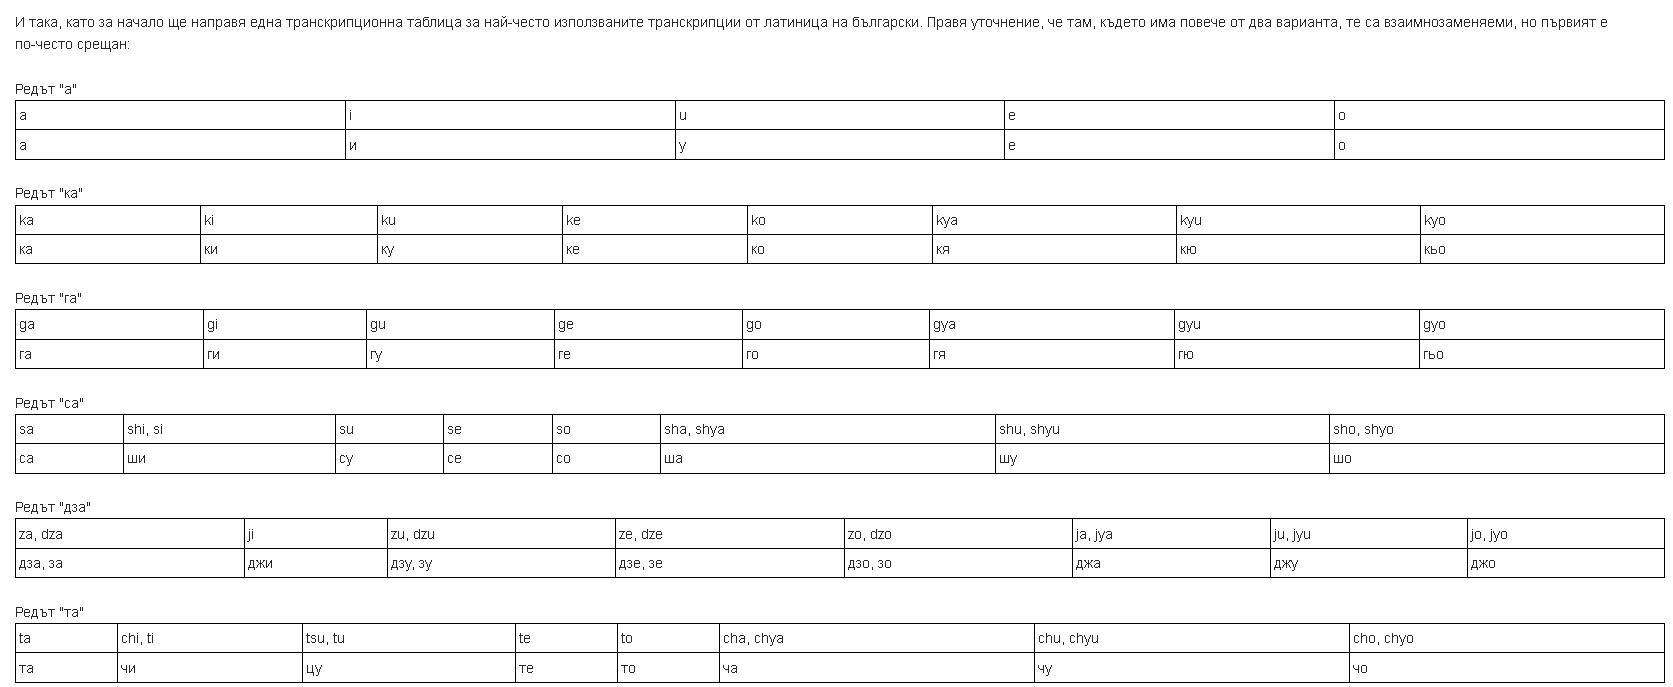
\includegraphics[width=\textwidth]{chapters/transcription-1.JPG}
    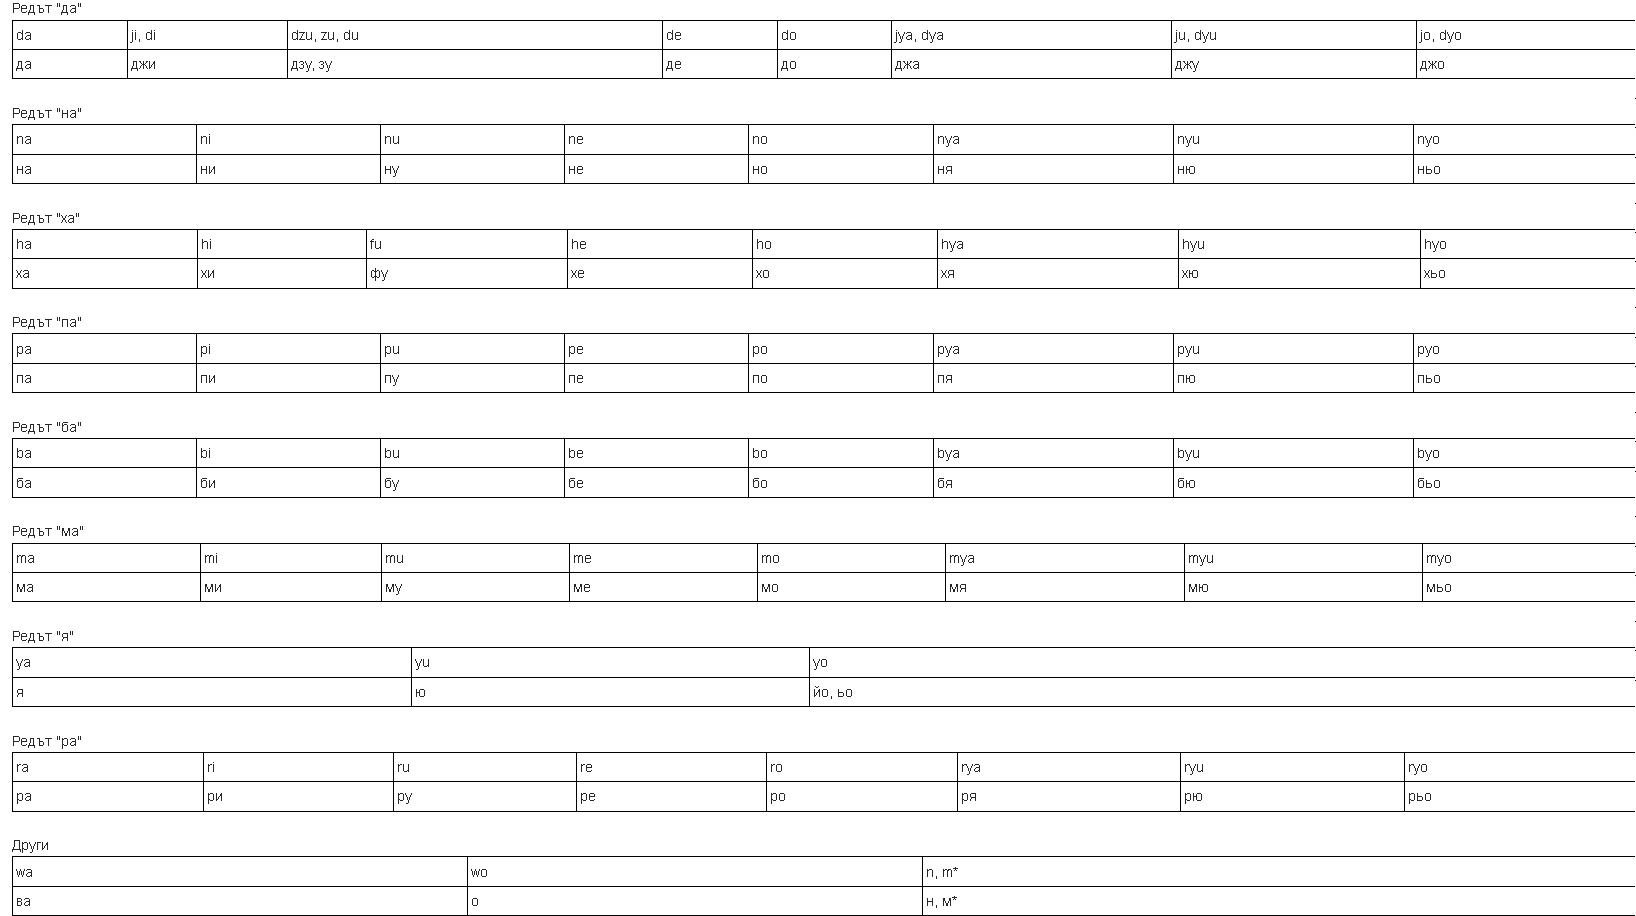
\includegraphics[width=\textwidth]{chapters/transcription-2.JPG}
    \caption{Транскрипционна таблица}
\end{table}

\clearpage

\section{Японски език за българи}
Следващата част е извадена от учебното пособие „Японски език за българи“ от Атанас Атанасов и Томоки Ватанабе.

\includepdf[pages={2-6},lastpage=24]{textbook.pdf} 
  
